\section{The circiut}

As mentioned in the text above the rover is consisted of six main components

\begin{table}[htbp]
    \caption{Components}
    \begin{center}
        \begin{tabular}{|c|c|}
            \hline
            \textbf{Component} & \textbf{No. of pieces}\\
            \hline
            STM32F103C8T6 & 1\\
            \hline
            KY-040 & 1\\
            \hline
            DC Motor & 4\\
            \hline
            L298N & 2\\
            \hline
            HC-05 & 1\\
            \hline
            HC-SR04 & 2\\
            \hline
        \end{tabular}
        \label{tab3}
    \end{center}
\end{table}

\subsection{Power}
Only components which are not connected to the microcontroller directly are the four DC motors. Power source for all the components is MCU's\footnote{MCU - Microcontroller Unit} 3.3V output. All the components share common grounding through the microcontroller. Secondary power source needed to run the motors is a 12V battery. 

\subsection{Scheme}

The scheme was created using a free open-source CAD software for the design of electronics hardware\footnote{https://fritzing.org}. As it hasn't been decided yet which type of battery will be used as a 12V power source for the motors to able to run propperly there is currently no real component in the figure \ref{fig6}. The components are connected using jumper wires with a 0.90mm diameter.
There is also an unused pin on the KY-040 encoder which acts as a button that triggers once the leaver of the rotary encoder is pushed\cite{KY-040}. L298N doesn't utilize its 5V input/output pin as it is not needed for the project.

\begin{figure}[htbp]
    \centerline{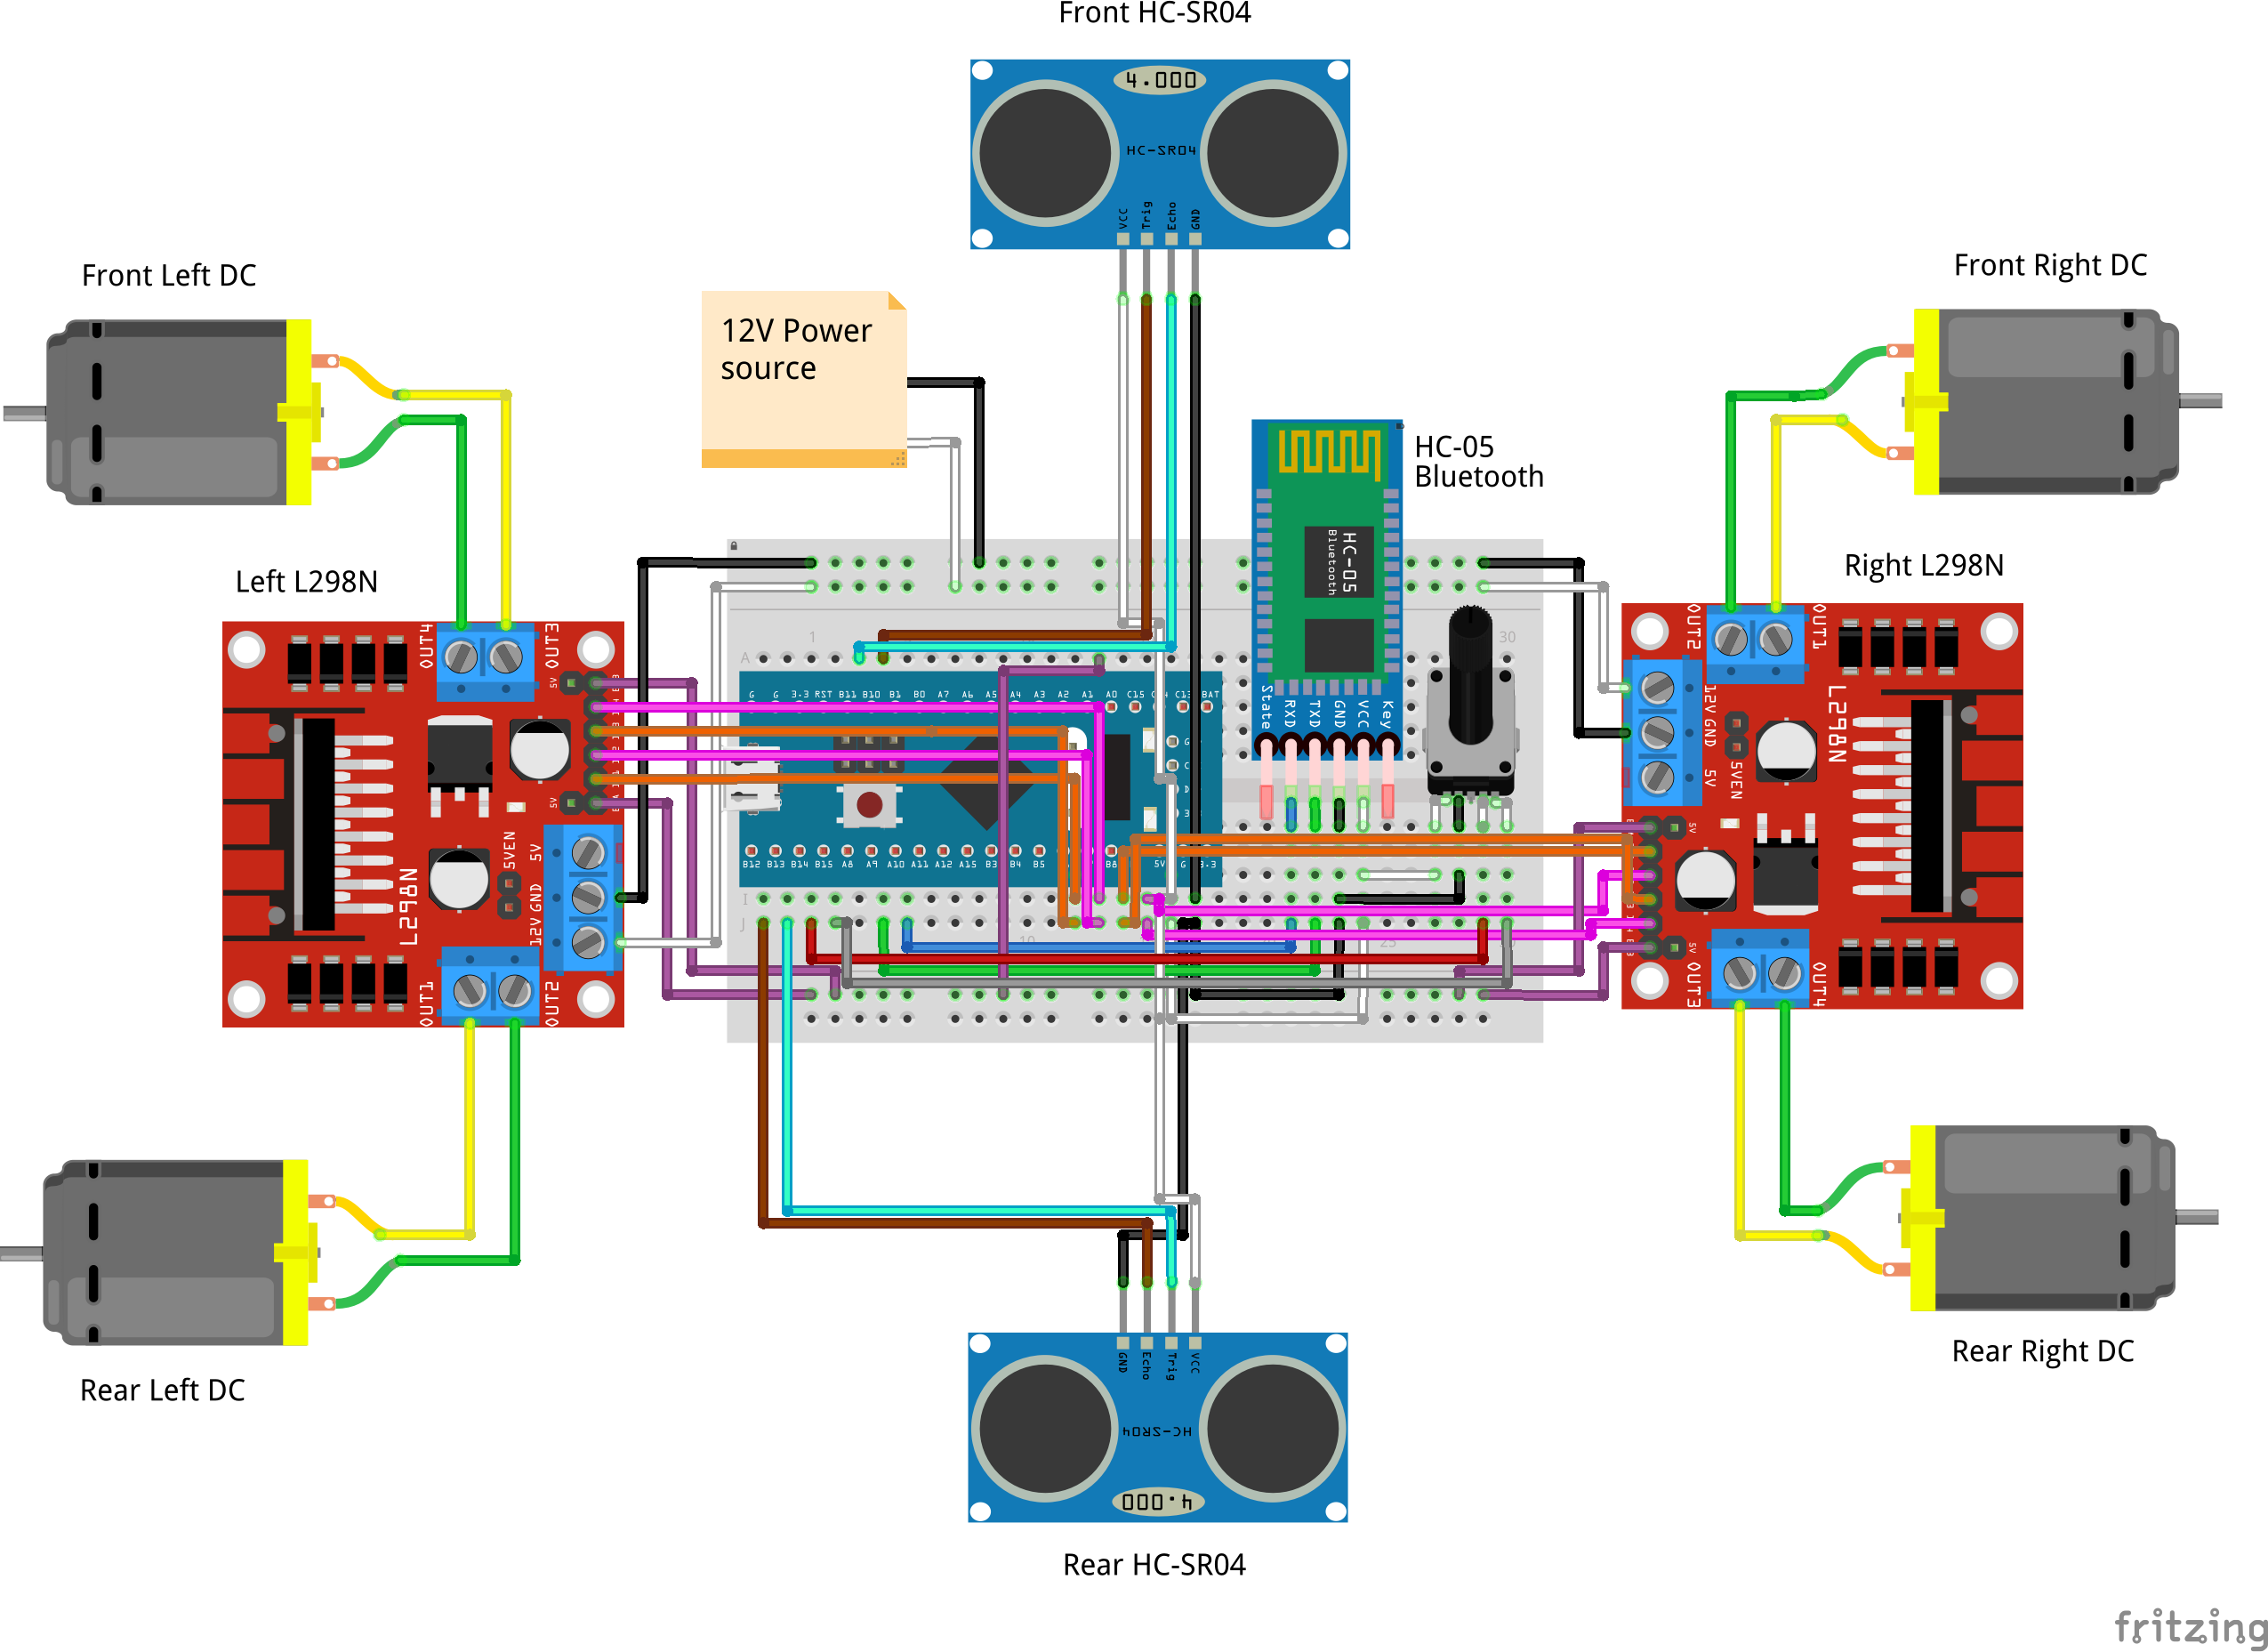
\includegraphics[width=8.5cm]{Images/Scheme.png}}
    \caption{Circuit Scheme}
    \label{fig6}
\end{figure}
 
The full list of connections in the scheme on figure \ref{fig6} can be seen in the table \ref{tab4}

\begin{table}[htbp]
    \caption{Component Connections}
    \begin{center}
        \begin{tabular}{|c|c|c|}
            \hline
            \textbf{Component} & \textbf{Pin} & \textbf{MCU pin}\\
            \hline
            KY-040 & CLK & B14/EXTI\\
            \hline
            KY-040 & DT & B15\\
            \hline
            Left L298N & IN1 & B6\\
            \hline
            Left L298N & IN2 & B7\\
            \hline
            Left L298N & IN3 & B6\\
            \hline
            Left L298N & IN4 & B7\\
            \hline
            Left L298N & EN1 & A1/PWM\\
            \hline
            Left L298N & EN2 & A1/PWM\\
            \hline
            Right L298N & IN1 & B8\\
            \hline
            Right L298N & IN2 & B9\\
            \hline
            Right L298N & IN3 & B8\\
            \hline
            Right L298N & IN4 & B9\\
            \hline
            Right L298N & EN1 & A1/PWM\\
            \hline
            Right L298N & EN2 & A1/PWM\\
            \hline
            HC-05 & RX & A9/TX\\
            \hline
            HC-05 & TX & A10/RX\\
            \hline
            Front HC-SR04 & TRIG & B25\\
            \hline
            Front HC-SR04 & ECHO & B26\\
            \hline
            Rear HC-SR04 & TRIG & B27\\
            \hline
            Rear HC-SR04 & ECHO & B28\\
            \hline
        \end{tabular}
        \label{tab4}
    \end{center}
\end{table}

The fritzing fzz file can be found on the projects Github page\footnote{https://www.github.com/Adi-Sose/Rover}.